% Reviewed translation: PDF pages 180--186 / printed pages 166--172.
% The original scan is authoritative; the duplicated source number (3.26) is preserved.
\MathBookSourcePage{180}

因此 \eqref{eq:primitive-q1-p0-summation-by-parts} 给出
\[
\begin{aligned}
\int_\Omega q\operatorname{div}\mathbf v\,dx
&=2h\sum_{i=-(n-1)}^{n-1}\sum_{j=-n}^{n-1}
\{v(2ih,(2j+1)h)-v(2ih,2jh)\}\\
&=h\sum_{i=-(n-1)}^{n-1}
\left\{\sum_{j=-n}^{n-1}\int_{2jh}^{(2j+1)h}
\frac{\partial v(2ih,x_2)}{\partial x_2}\,dx_2
-\sum_{j=-n+1}^{n}\int_{(2j-1)h}^{2jh}
\frac{\partial v(2ih,x_2)}{\partial x_2}\,dx_2\right\}.
\end{aligned}
\]
于是
\[
\begin{aligned}
\left|\int_\Omega q\operatorname{div}\mathbf v\,dx\right|
&\leq h\sum_{i=-(n-1)}^{n-1}\int_{-1}^{1}
\left|\frac{\partial v(2ih,x_2)}{\partial x_2}\right|dx_2\\
&\leq\sqrt2h(2n-1)^{1/2}
\left\{\int_{-1}^{1}\sum_{i=-(n-1)}^{n-1}
\left|\frac{\partial v(2ih,x_2)}{\partial x_2}\right|^2dx_2\right\}^{1/2}.
\end{aligned}
\]
注意, 对每个仿射函数 $f$, 下列求积公式成立:
\[
\int_0^1f^2(x)\,dx
=\frac13\{f^2(0)+f(0)f(1)+f^2(1)\}
\geq\frac14\max(f^2(0),f^2(1)),
\]
其中使用了不等式
\[
ab\leq\frac14a^2+b^2\qquad\forall a,b\geq0.
\]
因此
\[
\sum_{i=-(n-1)}^{n-1}
\left|\frac{\partial v(2ih,x_2)}{\partial x_2}\right|^2
\leq\frac2h\int_{-1}^{1}
\left|\frac{\partial v(x_1,x_2)}{\partial x_2}\right|^2dx_1.
\]
(这里使用了 $\partial v/\partial x_2$ 作为 $x_1$ 的函数是连续分片仿射函数这一事实.)
所以
\[
\left|\int_\Omega q\operatorname{div}\mathbf v\,dx\right|
\leq2(1-h)^{1/2}|\mathbf v|_{1,\Omega}.
\]
结合 \eqref{eq:primitive-q1-p0-counterexample-norm}, 得
\[
\left|\int_\Omega q\operatorname{div}\mathbf v\,dx\right|
/|\mathbf v|_{1,\Omega}
\leq\sqrt3h\|q\|_{0,\Omega}.
\]
由此证明如下结果.

\setcounter{statement}{5}
\renewcommand{\theHstatement}{lemma.\thesection.\arabic{statement}}
\begin{Lemma}\label{lem:primitive-q1-p0-sharpness}
在 Lemma~\ref{lem:primitive-q1-p0-degenerate-inf-sup} 的假设下,
由 \eqref{eq:primitive-q1-p0-counterexample-pressure} 定义的函数 $q$
属于 $\mathcal M_h$, 且满足

\MathBookSourcePage{181}
\[
\sup_{\mathbf v\in X_h}
\left[\left(\int_\Omega q\operatorname{div}\mathbf v\,dx\right)
/|\mathbf v|_{1,\Omega}\right]
\leq\sqrt3h\|q\|_{0,\Omega}.
\]
\end{Lemma}

与 Lemma~\ref{lem:primitive-q1-p0-degenerate-inf-sup} 合起来, 这说明常数
$\beta^*$ 确实为 $O(h)$.

事实上可以证明, 这个不理想的因子 $h$ 完全来自 $\mathcal M_h$ 中函数的
局部交替分量 $v_4$. 再次用基函数 $v_k$ 表示 $q\in\mathcal M_h$:
\[
q=\sum_{k=1}^{4}q^k,
\]
其中
\[
q^k=\sum_{I,J}(\alpha_kv_k)_{I,J},
\qquad(\alpha_k)_{I,J}\in\mathbb R,
\qquad\sum_{I,J}(\alpha_1)_{I,J}
=\sum_{I,J}(\alpha_4)_{I,J}=0.
\]
按照 Boland \& Nicolaides [12], 将 $\mathcal M_h$ 分解为
\[
\mathcal M_h=A_h+\widetilde M_h,
\]
其中
\begin{equation}\label{eq:primitive-q1-p0-pressure-decomposition}
\left\{
\begin{aligned}
A_h&=\{\,q\in\mathcal M_h;
\ q|_{\Omega_{I,J}}=(\alpha_4v_4)_{I,J}\,\},\\
\widetilde M_h=A_h^\perp
&=\{\,q\in\mathcal M_h;
\ q|_{\Omega_{I,J}}=(\alpha_1v_1+\alpha_2v_2+\alpha_3v_3)_{I,J}\,\}.
\end{aligned}
\right.
\end{equation}
并与这些空间联系 $X_h$ 的如下子空间:
\begin{equation}\label{eq:primitive-q1-p0-filtered-velocity-space}
\widetilde V_h=\{\,\mathbf v_h\in X_h;
\ (q_h,\operatorname{div}\mathbf v_h)=0
\quad\forall q_h\in A_h\,\}.
\end{equation}
我们要证明空间对 $(\widetilde V_h,\widetilde M_h)$ 满足一致 inf-sup 条件.
为此先建立一个局部条件.

\setcounter{statement}{6}
\renewcommand{\theHstatement}{lemma.\thesection.\arabic{statement}}
\begin{Lemma}\label{lem:primitive-q1-p0-macroelement-local-inf-sup}
采用上述记号和 Lemma~\ref{lem:primitive-q1-p0-degenerate-inf-sup} 的假设,
空间对 $(\widetilde V_h,\widetilde M_h)$ 关于 $\bar\Omega$ 的分割
$\{\Omega_{I,J}\}$ 一致满足局部 inf-sup 条件.
\end{Lemma}

\begin{Proof}
令
\[
X_h(\Omega_{I,J})
=\{\,\mathbf v\in\widetilde V_h;
\ \mathbf v|_{\partial\Omega_{I,J}}=0\,\},
\]
\[
M_h(\Omega_{I,J})
=\{\,q|_{\Omega_{I,J}};q\in\widetilde M_h\,\}
\cap L_0^2(\Omega_{I,J}).
\]
必须证明所有 $q\in M_h(\Omega_{I,J})$ 均满足
\begin{equation}\label{eq:primitive-q1-p0-macroelement-local-bound}
\sup_{\mathbf v\in X_h(\Omega_{I,J})}
\left[\left(\int_{\Omega_{I,J}}q\operatorname{div}\mathbf v\,dx\right)
/|\mathbf v|_{1,\Omega_{I,J}}\right]
\geq C\|q\|_{0,\Omega_{I,J}}.
\end{equation}
首先注意到
\[
X_h(\Omega_{I,J})
=\{\,\mathbf v=\mathbf v_{I,J}\phi_{I,J};
\ \mathbf v_{I,J}=(u_{I,J},v_{I,J})\in\mathbb R^2\,\},
\]
其中 $\phi_{I,J}$ 表示 $X_h$ 中在节点 $(I,J)$ 取值 $1$,
在 $\mathcal T_h$ 的所有其他节点取值 $0$ 的基函数. 类似地,

\MathBookSourcePage{182}
\[
M_h(\Omega_{I,J})
=\{\,q=\alpha_2(v_2)_{I,J}+\alpha_3(v_3)_{I,J};
\ \alpha_2,\alpha_3\in\mathbb R\,\}.
\]
于是对所有 $\mathbf v\in X_h(\Omega_{I,J})$ 和
$q\in M_h(\Omega_{I,J})$, 公式
\eqref{eq:primitive-q1-p0-summation-by-parts} 给出
\[
\int_{\Omega_{I,J}}q\operatorname{div}\mathbf v\,dx
=-2h(\alpha_2u_{I,J}+\alpha_3v_{I,J}),
\]
其中
\[
\|q\|_{0,\Omega_{I,J}}=2h(\alpha_2^2+\alpha_3^2)^{1/2}.
\]
取
\[
u_{I,J}=-2h\alpha_2,
\qquad v_{I,J}=-2h\alpha_3,
\]
立即得到 \eqref{eq:primitive-q1-p0-macroelement-local-bound},
其中 $C=(3/8)^{1/2}$.
\end{Proof}

令
\[
\bar M_h=\{\,q\in L_0^2(\Omega);
\ q|_{\Omega_{I,J}}\in\mathbb R\quad\forall I,J\,\}
=\{\,q\in\mathcal M_h;
\ q|_{\Omega_{I,J}}=(\alpha_1v_1)_{I,J}\,\}.
\]
由 Theorem~\ref{thm:primitive-local-to-global-inf-sup}, 若空间对
$(\widetilde V_h,\bar{\widetilde M}_h)$ 满足一致 inf-sup 条件,
则 $(\widetilde V_h,\widetilde M_h)$ 也满足. 后一个性质并不明显.
为证明它, 适宜将宏单元 $\Omega_{I,J}$ 按
Figure~\ref{fig:primitive-super-macroelement} 那样每四个分成一组;
当然必须假设这些超宏单元 $\mathcal O_{\alpha,\beta}$ 再次构成 $\Omega$ 的分割.
然后分两步进行. 首先引入 $\bar{\widetilde M}_h$ 的子空间
\[
\bar M_{2h}=\{\,q\in L_0^2(\Omega);
\ q|_{\mathcal O_{\alpha,\beta}}\in\mathbb R
\quad\forall\alpha,\beta\,\},
\]
并证明空间对 $(\widetilde V_h,\bar M_{2h})$ 满足一致 inf-sup 条件.
其次证明 $(\widetilde V_h,\bar{\widetilde M}_h)$ 在每个集合
$\mathcal O_{\alpha,\beta}$ 上满足局部 inf-sup 条件. 下面两个 Lemma 完成这些工作.

\begin{figure}[htbp]
\centering
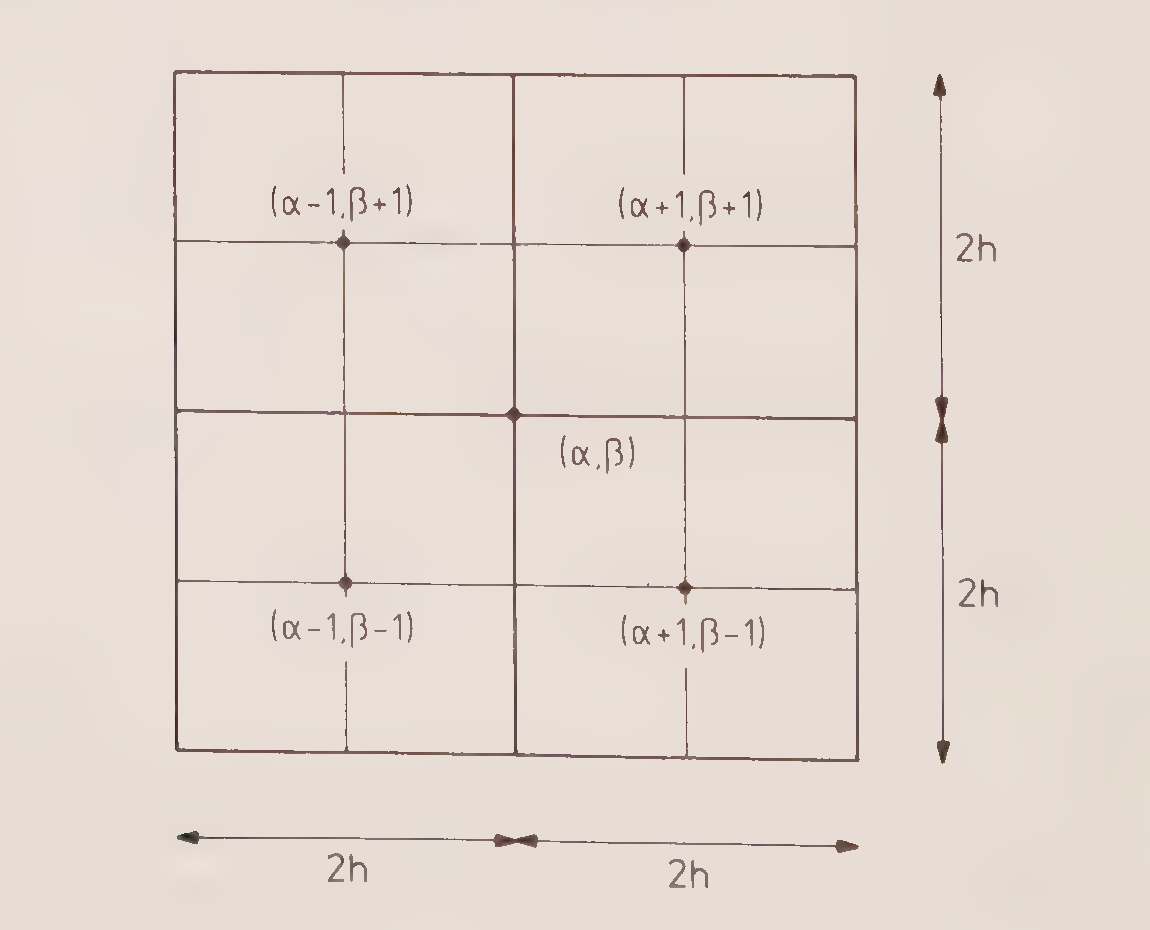
\includegraphics[width=.58\linewidth]{figures/chapter-02-figure-16.png}
\caption{超宏单元 $\mathcal O_{\alpha,\beta}$.}
\label{fig:primitive-super-macroelement}
\end{figure}

\MathBookSourcePage{183}
\setcounter{statement}{7}
\renewcommand{\theHstatement}{lemma.\thesection.\arabic{statement}}
\begin{Lemma}\label{lem:primitive-q1-p0-supermacro-global-inf-sup}
假设 $\bar\Omega$ 可以如 Figure~\ref{fig:primitive-super-macroelement}
所示, 分割为由四个宏单元 $\Omega_{I,J}$ 构成的各组
$\mathcal O_{\alpha,\beta}$. 则空间对
$(\widetilde V_h,\bar M_{2h})$ 满足全局一致 inf-sup 条件.
\end{Lemma}

\begin{Proof}
首先注意到 $X_{2h}$ 中的函数必定属于 $\widetilde V_h$, 因为它们的散度在每个
宏单元 $\Omega_{I,J}$ 上化为 $P_1$ 中的多项式, 并且
\[
\int_{\Omega_{I,J}}(v_4)_{I,J}p\,dx=0
\qquad\forall p\in P_1.
\]
因此只需证明空间对 $(X_{2h},\bar M_{2h})$ 的 inf-sup 条件.

为此构造一个与 Lemma~\ref{lem:primitive-bernardi-raugel-fortin-estimates}
中的算子非常相似的适当算子 $\pi_h$. 令 $R_h$ 是
Subsection~\ref{sec:appendix-interpolation-discontinuous-functions}
的局部正则化算子, 并固定一个超宏单元 $\mathcal O_{\alpha,\beta}$.
对 $v\in H^1(\mathcal O_{\alpha,\beta})$, 在每个
$\Omega_{I,J}\subset\mathcal O_{\alpha,\beta}$ 上定义 $\pi v\in Q_1$:
\[
\pi v(x_{i,j})=R_hv(x_{i,j})
\quad\text{于 $\mathcal O_{\alpha,\beta}$ 的四个角点和中心},
\]
\[
\int_T(\pi v-v)\,ds=0
\quad\text{于 $\partial\mathcal O_{\alpha,\beta}$ 的每条边 $T$}.
\]
然后在每个 $\mathcal O_{\alpha,\beta}$ 上取 $\pi_hv=\pi v$.
直接检验容易得到
$\pi_h\in\mathcal L(H_0^1(\Omega)^2;X_{2h})$, 且
\[
\int_\Omega\operatorname{div}(\pi_h\mathbf v-\mathbf v)q\,dx=0
\qquad\forall q\in\bar M_{2h}.
\]
此外, 一个简单论证表明
\[
|\pi_h\mathbf v|_{1,\Omega}\leq C|\mathbf v|_{1,\Omega},
\]
其中 $C>0$ 与 $h$ 无关. 这给出所需的 inf-sup 条件.
\end{Proof}

\setcounter{statement}{8}
\renewcommand{\theHstatement}{lemma.\thesection.\arabic{statement}}
\begin{Lemma}\label{lem:primitive-q1-p0-supermacro-local-inf-sup}
在每个 $\mathcal O_{\alpha,\beta}$ 上, 空间对
$(\widetilde V_h,\bar{\widetilde M}_h)$ 满足局部 inf-sup 条件.
\end{Lemma}

\begin{Proof}
设 $q$ 属于空间
\[
\bar M_h(\mathcal O_{\alpha,\beta})
=\{\,q|_{\mathcal O_{\alpha,\beta}}\,\}
\cap L_0^2(\mathcal O_{\alpha,\beta}).
\]
必须构造 $\widetilde V_h$ 中满足
$\mathbf v|_{\partial\mathcal O_{\alpha,\beta}}=0$ 的 $\mathbf v$, 使
\begin{equation}\label{eq:primitive-q1-p0-supermacro-local-bound}
\left(\int_{\mathcal O_{\alpha,\beta}}q\operatorname{div}\mathbf v\,dx\right)
/|\mathbf v|_{1,\mathcal O_{\alpha,\beta}}
\geq C\|q\|_{0,\mathcal O_{\alpha,\beta}}.
\end{equation}
在 $\mathcal O_{\alpha,\beta}$ 的边界和中心节点, 以及其所含每个宏单元
$\Omega_{I,J}$ 的中心节点, 固定 $\mathbf v=0$. 根据公式
\[
\int_{\mathcal O_{\alpha,\beta}}q\operatorname{div}\mathbf v\,dx
=-h^2\sum_{i,j}\{u_{i,j}(\nabla_1q)_{i,j}
+v_{i,j}(\nabla_2q)_{i,j}\},
\]

\MathBookSourcePage{184}
在 $\mathcal O_{\alpha,\beta}$ 其余所有节点 $(i,j)$ 上(即
$(\alpha\pm1,\beta),(\alpha,\beta\pm1)$)令
\[
u_{i,j}=-h(\nabla_1q)_{i,j},
\qquad v_{i,j}=-h(\nabla_2q)_{i,j}.
\]
容易看出, 对所有这些节点 $(i,j)$,
\[
(\nabla_kq^1)_{i,j}(\nabla_kq^4)_{i,j}=0,
\qquad k=1,2.
\]
因此所得函数 $\mathbf v$ 属于 $\widetilde V_h$, 并满足
\[
\int_{\mathcal O_{\alpha,\beta}}q\operatorname{div}\mathbf v\,dx
=h\sum_{i,j}\{|u_{i,j}|^2+|v_{i,j}|^2\}.
\]
于是 \eqref{eq:primitive-q1-p0-supermacro-local-bound} 由下列不等式得到:
\[
|\mathbf v_h|_{1,\mathcal O_{\alpha,\beta}}
\leq C_1\left(\sum_{i,j}\{|u_{i,j}|^2+|v_{i,j}|^2\}\right)^{1/2},
\]
其中 $C_1$ 与 $h,\alpha,\beta$ 无关, 以及
\[
\sum_{i,j}\{|u_{i,j}|^2+|v_{i,j}|^2\}
\geq2\sum_{I,J}|q_{I,J}|^2,
\]
这里考虑到 $q\in L_0^2(\mathcal O_{\alpha,\beta})$, 故
$\sum_{I,J}q_{I,J}=0$.
\end{Proof}

Lemmas~\ref{lem:primitive-q1-p0-macroelement-local-inf-sup}--
\ref{lem:primitive-q1-p0-supermacro-local-inf-sup} 立即给出下述结果.

\setcounter{statement}{3}
\renewcommand{\theHstatement}{theorem.\thesection.\arabic{statement}}
\begin{Theorem}\label{thm:primitive-q1-p0-filtered-inf-sup}
假设 $\Omega$ 可如 Figure~\ref{fig:primitive-super-macroelement}
所示, 分割为由四个宏单元组成的各组 $\mathcal O_{\alpha,\beta}$.
则由 \eqref{eq:primitive-q1-p0-filtered-velocity-space} 和
\eqref{eq:primitive-q1-p0-pressure-decomposition} 定义的空间对
$(\widetilde V_h,\widetilde M_h)$ 满足一致 inf-sup 条件.
\end{Theorem}

\setcounter{statement}{0}
\renewcommand{\theHstatement}{remark.\thesection.\arabic{statement}}
\begin{Remark}\label{rem:primitive-q1-p0-xh-bar-mh}
Lemma~\ref{lem:primitive-q1-p0-supermacro-global-inf-sup} 的论证可直接用于证明
空间对 $(X_h,\bar M_h)$ 满足一致 inf-sup 条件, 但这并不蕴含
$(\widetilde V_h,\bar M_h)$ 也满足该条件.
\end{Remark}

\setcounter{statement}{1}
\renewcommand{\theHstatement}{remark.\thesection.\arabic{statement}}
\begin{Remark}\label{rem:primitive-q1-p0-general-quadrilaterals}
上述分析不能直接用于任意四边形. 通常, ``棋盘格''伪压力会从 $M_h$ 中消失,
但 inf-sup 条件仍不满足(见 Sani et al. [70]). 不过, 对于特殊四边形网格,
可以导出类似结果(见 Pitkäranta \& Stenberg [65]).
\end{Remark}

\subsection{$Q_1$--$P_0$ 单元的误差估计}
\label{subsec:primitive-q1-p0-error-estimates}

本小节旨在证明: 虽然空间对 $(X_h,M_h)$ 不满足 inf-sup 条件,
仍可用它成功计算速度 $\mathbf u$, 并且在采取某些预防措施时计算压力 $p$.
为此, Theorem~\ref{thm:primitive-q1-p0-filtered-inf-sup} 的陈述将起关键作用.

设 $(\mathbf u_h,p_h)\in X_h\times M_h$ 是下列问题的一个解:

\MathBookSourcePage{185}
\begin{equation*}
\tag{3.26}\label{eq:primitive-q1-p0-discrete-system-source-number}
\left\{
\begin{aligned}
\nu(\operatorname{grad}\mathbf u_h,\operatorname{grad}\mathbf v_h)
-(p_h,\operatorname{div}\mathbf v_h)
&=\langle\mathbf f,\mathbf v_h\rangle
&&\forall\mathbf v_h\in X_h,\\
(q_h,\operatorname{div}\mathbf u_h)&=0
&&\forall q_h\in M_h,
\end{aligned}
\right.
\end{equation*}
其中 $X_h,M_h$ 由 \eqref{eq:primitive-q1-p0-spaces} 定义.
我们知道 $\mathbf u_h$ 是唯一的, 但每个 $p_h$ 都具有形式
\[
p_h=\tilde p_h+p_h^4+C\mu,
\]
其中 $\mu$ 由 \eqref{eq:primitive-checkerboard-function} 定义,
$p_h^4$ 和 $\tilde p_h$ 分别在 $A_h$ 和 $\widetilde M_h$ 中唯一确定,
$C$ 则为任意常数. 此外, $\mathbf u_h\in\widetilde V_h$,
其中 $\widetilde V_h$ 由 \eqref{eq:primitive-q1-p0-filtered-velocity-space} 定义,
且空间对 $(\mathbf u_h,\tilde p_h)\in\widetilde V_h\times\widetilde M_h$
是下列问题的唯一解:
\setcounter{equation}{36}
\begin{equation}\label{eq:primitive-q1-p0-filtered-discrete-system}
\left\{
\begin{aligned}
\nu(\operatorname{grad}\mathbf u_h,\operatorname{grad}\tilde{\mathbf v}_h)
-(\tilde p_h,\operatorname{div}\tilde{\mathbf v}_h)
&=\langle\mathbf f,\tilde{\mathbf v}_h\rangle
&&\forall\tilde{\mathbf v}_h\in\widetilde V_h,\\
(\tilde q_h,\operatorname{div}\mathbf u_h)&=0
&&\forall\tilde q_h\in\widetilde M_h.
\end{aligned}
\right.
\end{equation}
因此, 由 Theorem~\ref{thm:primitive-q1-p0-filtered-inf-sup},
可直接把 Theorem~\ref{thm:primitive-abstract-discrete-error} 2)用于
$\widetilde V_h,\widetilde M_h$, 分别替代 $X_h,M_h$:
\begin{equation}\label{eq:primitive-q1-p0-quasi-optimal-error}
\left\{
\begin{aligned}
&|\mathbf u-\mathbf u_h|_{1,\Omega}
+\|p-\tilde p_h\|_{0,\Omega}\\
&\qquad\leq C_1\left\{
\inf_{\tilde{\mathbf v}_h\in\widetilde V_h}
|\mathbf u-\tilde{\mathbf v}_h|_{1,\Omega}
+\inf_{\tilde q_h\in\widetilde M_h}
\|p-\tilde q_h\|_{0,\Omega}\right\},
\end{aligned}
\right.
\end{equation}
其中常数 $C_1>0$ 与 $h$ 无关.

于是还需研究空间 $\widetilde V_h,\widetilde M_h$ 的逼近性质.
对 $\widetilde V_h$, 回忆(见
Lemma~\ref{lem:primitive-q1-p0-supermacro-global-inf-sup})
\[
X_{2h}\subset\widetilde V_h.
\]
因此 \eqref{eq:appendix-quadrilateral-lagrange-error-wsp} 给出
\begin{equation}\label{eq:primitive-q1-p0-velocity-approximation}
\inf_{\tilde{\mathbf v}_h\in\widetilde V_h}
|\mathbf u-\tilde{\mathbf v}_h|_{1,\Omega}
\leq|\mathbf u-I_{2h}\mathbf u|_{1,\Omega}
\leq C_2h|\mathbf u|_{2,\Omega}
\qquad\forall\mathbf u\in H^2(\Omega)^2.
\end{equation}
类似地, 由于 $\bar M_h\subset\widetilde M_h$,
\eqref{eq:appendix-quadrilateral-l2-projection} 给出
\begin{equation}\label{eq:primitive-q1-p0-pressure-approximation}
\inf_{\tilde q_h\in\widetilde M_h}\|p-\tilde q_h\|_{0,\Omega}
\leq\|p-\rho_{2h}p\|_{0,\Omega}
\leq C_3h|p|_{1,\Omega}
\qquad\forall p\in H^1(\Omega).
\end{equation}
这三个不等式汇成如下 Theorem.

\setcounter{statement}{4}
\renewcommand{\theHstatement}{theorem.\thesection.\arabic{statement}}
\begin{Theorem}\label{thm:primitive-q1-p0-error}
设 $\Omega$ 与 Theorem~\ref{thm:primitive-q1-p0-filtered-inf-sup} 中相同,
并假设 Stokes 系统的解 $(\mathbf u,p)$ 满足
\[
\mathbf u\in[H^2(\Omega)\cap H_0^1(\Omega)]^2,
\qquad p\in H^1(\Omega)\cap L_0^2(\Omega).
\]
则格式 \eqref{eq:primitive-q1-p0-discrete-system-source-number} 的解
$(\mathbf u_h,p_h)$ 满足误差估计
\begin{equation}\label{eq:primitive-q1-p0-h1-pressure-error}
|\mathbf u-\mathbf u_h|_{1,\Omega}
+\|p-\tilde p_h\|_{0,\Omega}
\leq Ch\{\|\mathbf u\|_{2,\Omega}+|p|_{1,\Omega}\},
\end{equation}
其中 $\tilde p_h$ 是 $p_h$ 在 $\widetilde M_h$ 中的分量.
\end{Theorem}

$\tilde p_h$ 分量充当压力 $p_h$ 的滤波器, 因为它完全舍弃交替函数 $v_4$.
由 Lemma~\ref{lem:primitive-q1-p0-sharpness} 可知, 对整个 $p_h$ 不能期待令人满意的估计.

\MathBookSourcePage{186}
不过, 我们将看到 $p_h$ 在 $A_h$ 中的补充分量 $p_h^4$ 是有界的.
事实上, 由 \eqref{eq:primitive-q1-p0-discrete-system-source-number} 得
\[
(p_h^4,\operatorname{div}\mathbf v_h)
=\nu(\operatorname{grad}(\mathbf u_h-\mathbf u),
\operatorname{grad}\mathbf v_h)
+(p-\tilde p_h,\operatorname{div}\mathbf v_h)
\qquad\forall\mathbf v_h\in X_h.
\]
所以
\[
\sup_{\mathbf v_h\in X_h}
\left[\frac{(p_h^4,\operatorname{div}\mathbf v_h)}
{|\mathbf v_h|_{1,\Omega}}\right]
\leq C_4h\{\|\mathbf u\|_{2,\Omega}+|p|_{1,\Omega}\}.
\]
在最好情形下, 该不等式左端可能由
$C_5\|p_h^4\|_{0,\Omega}$ 从下方控制, 其中 $C_5$ 与 $h$ 无关,
于是 $\|p_h^4\|_{0,\Omega}$ 为 $O(h)$. 但在一般情形中, 只能应用
Lemma~\ref{lem:primitive-q1-p0-degenerate-inf-sup}, 得到如下结果.

\setcounter{statement}{0}
\renewcommand{\theHstatement}{corollary.\thesection.\arabic{statement}}
\begin{Corollary}\label{cor:primitive-q1-p0-spurious-pressure-bound}
在 Theorem~\ref{thm:primitive-q1-p0-error} 的假设下,
$p_h$ 在 $A_h$ 中的分量 $p_h^4$ 满足
\begin{equation}\label{eq:primitive-q1-p0-spurious-pressure-bound}
\|p_h^4\|_{0,\Omega}
\leq C\{\|\mathbf u\|_{2,\Omega}+|p|_{1,\Omega}\}.
\end{equation}
\end{Corollary}

最后, 还可对空间对 $(\widetilde V_h,\widetilde M_h)$ 应用
Theorem~\ref{thm:primitive-duality-error}, 导出
$\|\mathbf u-\mathbf u_h\|_{0,\Omega}$ 的最优误差估计.

\setcounter{statement}{1}
\renewcommand{\theHstatement}{corollary.\thesection.\arabic{statement}}
\begin{Corollary}\label{cor:primitive-q1-p0-l2-error}
在 Theorem~\ref{thm:primitive-q1-p0-error} 的假设下, 有
\begin{equation}\label{eq:primitive-q1-p0-l2-error}
\|\mathbf u-\mathbf u_h\|_{0,\Omega}
\leq Ch^2\{\|\mathbf u\|_{2,\Omega}+|p|_{1,\Omega}\}.
\end{equation}
\end{Corollary}

\begin{figure}[htbp]
\centering
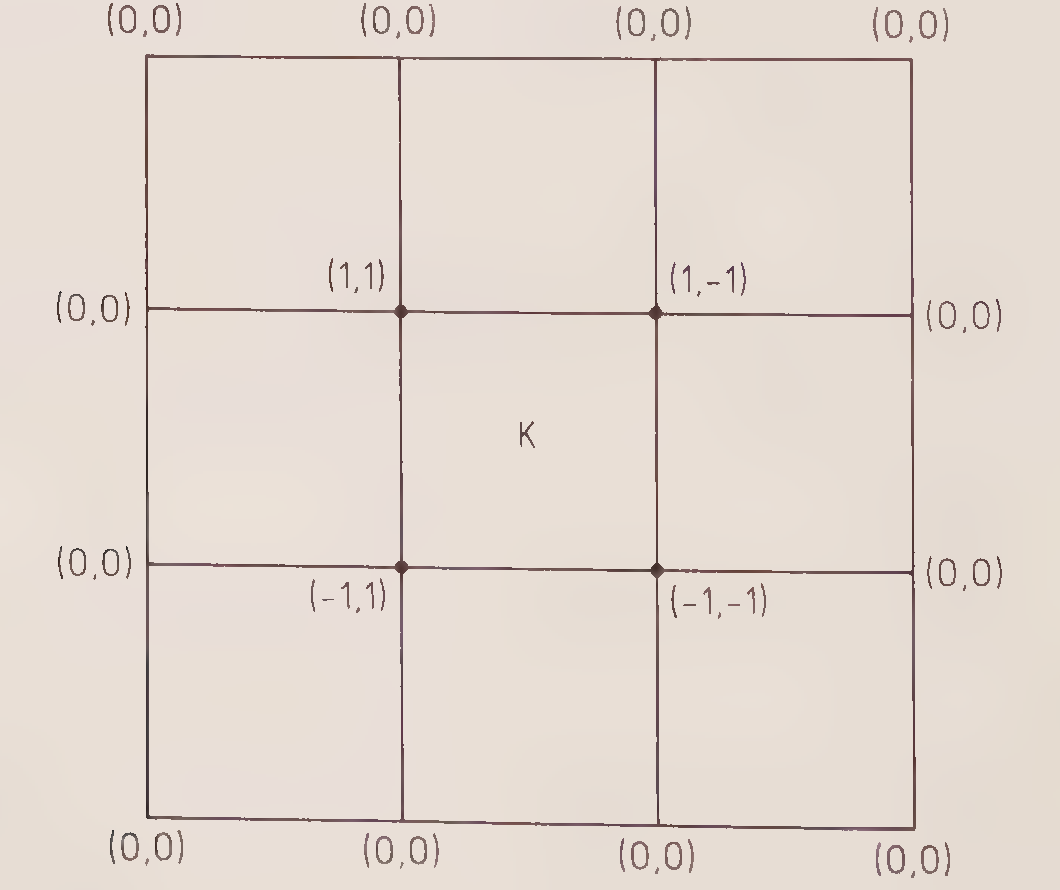
\includegraphics[width=.55\linewidth]{figures/chapter-02-figure-17.png}
\caption{$Q_1$--$P_0$ 速度节点值的局部图案.}
\label{fig:primitive-q1-p0-local-velocity-pattern}
\end{figure}

\MathBookSourcePage{187}
数值结果证实了上述理论分析, 但最常见的情形似乎是整个压力 $p_h$
趋于 $p$, 而不仅是分量 $\tilde p_h$. 因而通常没有必要滤除压力分量
$p_h^4$. 不过, 在某些情形下 $p_h^4$ 确实发散; 具体例子可参见
Boland \& Nicolaides. 此外, Malkus \& Olsen
还给出了其他一些目前仍在使用、但不满足一致 inf-sup 条件的有限元空间例子.

从实际计算的观点看, 问题
\eqref{eq:primitive-q1-p0-discrete-system-source-number} 可用
Subsection~\ref{subsec:primitive-homogeneous-stokes} 的惩罚方法求解
(参见 \eqref{eq:primitive-stokes-penalty-problem}). 例如, Carey \& Krishnan
给出了数值结果. 但是, 也可以使用“无散度”速度空间 $V_h$ 的一组基,
直接把速度与压力解耦. 按照 Stephens et al., 对每个单元 $\kappa$,
引入向量场 $\mathbf v_\kappa\in X_h$: 它在 $\kappa$ 的四个顶点上分别取值
$(1,-1)$, $(1,1)$, $(-1,1)$, $(-1,-1)$, 如
Figure~\ref{fig:primitive-q1-p0-local-velocity-pattern} 所示, 并在
$\mathcal T_h$ 的所有其他节点上取值 $(0,0)$. 定义
\[
S=\{\mathbf v_\kappa;\ \kappa\text{ 为 }\mathcal T_h\text{ 的内部单元}\}.
\]
直接检查即可确认, $S$ 中每个 $\mathbf v_\kappa$ 都属于 $V_h$, 且这些函数
线性无关. 此外, 简单的维数论证给出
\[
\operatorname{card}(S)=\dim(X_h)-\dim(\mathcal M_h)=\dim(V_h).
\]
因此 $S$ 是 $V_h$ 的一组方便的基. 上述文献给出了使用这组基的数值结果.
